\documentclass[english,floatsintext,man]{apa6}

\usepackage{amssymb,amsmath}
\usepackage{ifxetex,ifluatex}
\usepackage{fixltx2e} % provides \textsubscript
\ifnum 0\ifxetex 1\fi\ifluatex 1\fi=0 % if pdftex
  \usepackage[T1]{fontenc}
  \usepackage[utf8]{inputenc}
\else % if luatex or xelatex
  \ifxetex
    \usepackage{mathspec}
    \usepackage{xltxtra,xunicode}
  \else
    \usepackage{fontspec}
  \fi
  \defaultfontfeatures{Mapping=tex-text,Scale=MatchLowercase}
  \newcommand{\euro}{€}
\fi
% use upquote if available, for straight quotes in verbatim environments
\IfFileExists{upquote.sty}{\usepackage{upquote}}{}
% use microtype if available
\IfFileExists{microtype.sty}{\usepackage{microtype}}{}

% Table formatting
\usepackage{longtable,booktabs}
\usepackage[counterclockwise]{rotating}   % Landscape page setup for large tables
\usepackage{multirow}		% Table styling
\usepackage{tabularx}		% Control Column width
\usepackage[flushleft]{threeparttable}	% Allows for three part tables with a specified notes section
\usepackage{threeparttablex}            % Lets threeparttable work with longtable
\usepackage{longtable}              % Allows tables to break across pages

  \usepackage{graphicx}
  \makeatletter
  \def\maxwidth{\ifdim\Gin@nat@width>\linewidth\linewidth\else\Gin@nat@width\fi}
  \def\maxheight{\ifdim\Gin@nat@height>\textheight\textheight\else\Gin@nat@height\fi}
  \makeatother
  % Scale images if necessary, so that they will not overflow the page
  % margins by default, and it is still possible to overwrite the defaults
  % using explicit options in \includegraphics[width, height, ...]{}
  \setkeys{Gin}{width=\maxwidth,height=\maxheight,keepaspectratio}
\ifxetex
  \usepackage[setpagesize=false, % page size defined by xetex
              unicode=false, % unicode breaks when used with xetex
              xetex]{hyperref}
\else
  \usepackage[unicode=true]{hyperref}
\fi
\hypersetup{breaklinks=true,
            pdfauthor={},
            pdftitle={A Quantitative Synthesis of Early Language Acquisition Using Meta-Analysis},
            colorlinks=true,
            citecolor=blue,
            urlcolor=blue,
            linkcolor=black,
            pdfborder={0 0 0}}
\urlstyle{same}  % don't use monospace font for urls

\setlength{\parindent}{0pt}
%\setlength{\parskip}{0pt plus 0pt minus 0pt}

\setlength{\emergencystretch}{3em}  % prevent overfull lines

\setcounter{secnumdepth}{0}
\ifxetex
  \usepackage{polyglossia}
  \setmainlanguage{}
\else
  \usepackage[english]{babel}
\fi

% Manuscript styling
\captionsetup{font=singlespacing,justification=justified}
\usepackage{csquotes}



\usepackage{tikz} % Variable definition to generate author note

% fix for \tightlist problem in pandoc 1.14
\providecommand{\tightlist}{%
  \setlength{\itemsep}{0pt}\setlength{\parskip}{0pt}}

% Essential manuscript parts
  \title{A Quantitative Synthesis of Early Language Acquisition Using
Meta-Analysis}

  \shorttitle{A Quantitative Synthesis}


  \author{
          Molly Lewis\textsuperscript{1},
          Mika Braginsky\textsuperscript{1},
          Sho Tsuji\textsuperscript{2},
          Christina Bergmann\textsuperscript{2},
          Page Piccinini\textsuperscript{2},
          Alejandrina Cristia\textsuperscript{2},
          Michael C. Frank\textsuperscript{1}  }

  \def\affdep{{"", "", "", "", "", "", ""}}%
  \def\affcity{{"", "", "", "", "", "", ""}}%

  \affiliation{
    \vspace{0.5cm}
          \textsuperscript{1} Department Psychology, Stanford University\\
          \textsuperscript{2} Laboratoire de Sciences Cognitives et Psycholinguistique, ENS  }


%   \def\affinst{{"init", "Department Psychology, Stanford University", "Laboratoire de Sciences Cognitives et Psycholinguistique, ENS"}}%
%   \def\affstate{{"init", "", ""}}%
%   \def\affcntry{{"init", "", ""}}%

  \note{
    \vspace{1cm}
    Author note

    \raggedright
    \setlength{\parindent}{0.4in}

    \newcounter{author}

%     %     %       %       \setcounter{author}{0}
%         %           \addtocounter{author}{1}
%         %         \expandafter\edef\csname authorid\endcsname{\theauthor}
%         Molly Lewis, \pgfmathparse{\affdep[\authorid]} \pgfmathresult, \pgfmathparse{\affinst[\authorid]} \pgfmathresult, \pgfmathparse{\affcity[\authorid]} \pgfmathresult, \pgfmathparse{\affstate[\authorid]} \pgfmathresult, \pgfmathparse{\affcntry[\authorid]} \pgfmathresult
%       %     ;
%     %       %       \setcounter{author}{0}
%         %           \addtocounter{author}{1}
%         %         \expandafter\edef\csname authorid\endcsname{\theauthor}
%         Mika Braginsky, \pgfmathparse{\affdep[\authorid]} \pgfmathresult, \pgfmathparse{\affinst[\authorid]} \pgfmathresult, \pgfmathparse{\affcity[\authorid]} \pgfmathresult, \pgfmathparse{\affstate[\authorid]} \pgfmathresult, \pgfmathparse{\affcntry[\authorid]} \pgfmathresult
%       %     ;
%     %       %       \setcounter{author}{0}
%         %           \addtocounter{author}{2}
%         %         \expandafter\edef\csname authorid\endcsname{\theauthor}
%         Sho Tsuji, \pgfmathparse{\affdep[\authorid]} \pgfmathresult, \pgfmathparse{\affinst[\authorid]} \pgfmathresult, \pgfmathparse{\affcity[\authorid]} \pgfmathresult, \pgfmathparse{\affstate[\authorid]} \pgfmathresult, \pgfmathparse{\affcntry[\authorid]} \pgfmathresult
%       %     ;
%     %       %       \setcounter{author}{0}
%         %           \addtocounter{author}{2}
%         %         \expandafter\edef\csname authorid\endcsname{\theauthor}
%         Christina Bergmann, \pgfmathparse{\affdep[\authorid]} \pgfmathresult, \pgfmathparse{\affinst[\authorid]} \pgfmathresult, \pgfmathparse{\affcity[\authorid]} \pgfmathresult, \pgfmathparse{\affstate[\authorid]} \pgfmathresult, \pgfmathparse{\affcntry[\authorid]} \pgfmathresult
%       %     ;
%     %       %       \setcounter{author}{0}
%         %           \addtocounter{author}{2}
%         %         \expandafter\edef\csname authorid\endcsname{\theauthor}
%         Page Piccinini, \pgfmathparse{\affdep[\authorid]} \pgfmathresult, \pgfmathparse{\affinst[\authorid]} \pgfmathresult, \pgfmathparse{\affcity[\authorid]} \pgfmathresult, \pgfmathparse{\affstate[\authorid]} \pgfmathresult, \pgfmathparse{\affcntry[\authorid]} \pgfmathresult
%       %     ;
%     %       %       \setcounter{author}{0}
%         %           \addtocounter{author}{2}
%         %         \expandafter\edef\csname authorid\endcsname{\theauthor}
%         Alejandrina Cristia, \pgfmathparse{\affdep[\authorid]} \pgfmathresult, \pgfmathparse{\affinst[\authorid]} \pgfmathresult, \pgfmathparse{\affcity[\authorid]} \pgfmathresult, \pgfmathparse{\affstate[\authorid]} \pgfmathresult, \pgfmathparse{\affcntry[\authorid]} \pgfmathresult
%       %     ;
%     %       %       \setcounter{author}{0}
%         %           \addtocounter{author}{1}
%         %         \expandafter\edef\csname authorid\endcsname{\theauthor}
%         Michael C. Frank, \pgfmathparse{\affdep[\authorid]} \pgfmathresult, \pgfmathparse{\affinst[\authorid]} \pgfmathresult, \pgfmathparse{\affcity[\authorid]} \pgfmathresult, \pgfmathparse{\affstate[\authorid]} \pgfmathresult, \pgfmathparse{\affcntry[\authorid]} \pgfmathresult
%       %     .
%     
    Correspondence concerning this article should be addressed to Molly
    Lewis, Psychology Department, Stanford University. 450 Serra Mall,
    Stanford, CA 94305. E-mail:
    \href{mailto:mll@stanford.edu}{\nolinkurl{mll@stanford.edu}}.

                                                                                    }

  \abstract{replicability, etc.}
  \keywords{replicability, reproducibility, meta-analysis, developmental psychology,
language acquisition \\

    \indent Word count: XXXX
  }

  \usepackage{setspace}
  \usepackage{float}
  \usepackage{graphicx}
  \AtBeginEnvironment{tabular}{\singlespacing}
  \usepackage{pbox}

\begin{document}

\maketitle



\section{Introduction}\label{introduction}

To learn to speak a language, a child must acquire a wide range
knowledge and skills: the sounds of the language, the word forms, and
how words map to meanings, to name only a few. How does this process
unfold? Our goal as psychologists is to build a theory that can explain
and predict this process in a way that is both precise but also highly
generalizable. The challenge we face, however, is that we must build
this theory on the basis of very limited data, and, as a consequence, we
must rely on error-prone inductive reasoning strategies to build our
theories. In this paper, we consider the domain of language acquisition
and demonstrate how meta-analytic methods can support the inductive
theory-building process.

Meta-analysis is a quantitative method for aggregating across
experimental findings. The fundamental unit of meta-analysis is the
\emph{effect size}: a scale-free, quantitative measure of
\enquote{success} in a phenomenon. Importantly, an effect size provides
an estimate of the \emph{size} of an effect, as well as a measure of
uncertainty around this point estimate. With such a quantitative measure
of success, we can apply the same reasoning we use to aggregate noisy
measurements over participants in a single study: By assuming each
\emph{study}, rather than participant, is sampled from a population, we
can appeal to the classical statistical framework to combine estimates
of the effect size for a given phenomenon.

Meta-analytic methods support theory building in several ways. First,
they provide a way of evaluating which effects in a literature are
\enquote{real,} and thus should constrain the theory. This is
particularly important in light of recent high-profile evidence in the
field that an effect observed in one study may not replicate in another
(``replication crisis,'' Ioannidis, 2005; Open Science Collaboration,
2012, 2015). Failed replications are difficult to interpret, however,
because they may result from a wide variety of causes, including an in
initial false positive, a subsequent false negative, or differences
between initial and replication studies, and making causal attributions
in a situation with two conflicting studies is often difficult (Anderson
et al., 2016; Gilbert, King, Pettigrew, \& Wilson, 2016). Meta-analysis
can allow researchers to address this set of issues in a principled way
by aggregating evidence across studies and assuming that there is some
variability in true effect size from study to study. In this way,
meta-analytic methods can provide more veridical description of the
empirical landscape, which in turn leads to better theory-building.

Second, meta-analysis supports theory building by providing higher
fidelity descriptions of phenomena. In addition to providing a
quantitative estimate of success, meta-analytic methods provide a method
for quantifying the amount variability around this point estimate.
Furthermore, the quantitative framework allows researchers to detect
potential moderators in effect size. This is particularly important for
developmental phenomena because building a theory requires, critically,
a clear description of the changes in effect size across development.
Typically, individual papers describe an effect size within the same
paradigm, across 1-3 age groups. To the extent that the effect size at
\emph{each} of these developmental timepoints is a noisy sample from the
true underlying effect size, it may be quite difficult to detect
developmental trends in effect sizes from individual papers. By
aggregating across papers through meta-analytic methods, however, we can
provide a more precise description of the empirical phenomena.

In addition to providing a quantiative measure of success, effect size
estimates also provide a common language for comparing \emph{across}
phenomena. This common language allows us to meaningfully consider the
relationship between different phenomena in the language acquisition
domain (\enquote{meta-meta-analysis}). Through cross-phenomena
comparisons, we can understand not only the trajectory of a particular
phenomenon, like word learning for example, but also how this phenomenon
might depend on other skills, such as sound learning, gaze following,
and many others.

Finally, in addition to these theoretical motivations, there are
practical reasons for conducting a quantitative synthesis. When planning
an experiment, an estimate of the size of an effect on the basis of
prior literature can inform the sample size needed to achieve a desired
level of power. Meta-analytic estimates of effect sizes can also aid in
design choices: If a certain paradigm tends to have overall larger
effect sizes than another, the strategic researcher might select this
paradigm in order to maximize the power of a study.

While meta-analytic methods are likely helpful for many psychological
literatures, we believe language acquisition is a particularly
informative application for this tool. One reason is that language
acquisition may be uniquely vulnerable to false findings because running
children is expensive, and thus sample sizes are small and studies are
underpowered (Ioannidis, 2005). In addition, the difficulty in running
participants means that replications are relatively rare in the field.
Finally, there has been attention to developmental psychology research
practices more broadly, suggesting evidence of experimenter bias
(Peterson, 2016).

We take as our ultimate goal a single overarching theory of language
acquisition that can explain and predict all the relevant phenomena.
Toward this end, we developed a dataset of effect sizes in the language
acquisition literature across 12 different phenomena
(\href{http://metalab.stanford.edu}{Metalab;
http://metalab.stanford.edu/}). We demonstrate how meta-analysis
supports building this theory in two ways. We first use meta-analytic
techniques to evaluate the evidential value of the empirical landscape
in language acquisition research. We find broadly that this literature
has strong evidential value, and thus that the effects report in the
literature should constrain our theory of language acquisition. We then
turn to synthesizing these findings across phenomena and offer a
preliminary theoretical synthesis of the field.

\section{Method}\label{method}

We analyzed 12 different phenomena in language acquisition. These
phenomena were selected opportunistically, based on their availability
in the literature and feasibility of conducting meta-analysis for a
particular phenomenon. The phenomena cover development at many different
levels of the language hierarchy, from the acquisition of prosody and
phonemic contrasts, to gaze following in linguistic interaction. This
wide range of phenomena allowed us to compare the course of development
across different domains, as well as explore questions about the
interactive nature of language acquisition (Table 1).

To obtain estimates of effect size, we coded papers reporting
experimental data. Within each paper, we calculated a separate effect
size estimate for each experiment and age group (\enquote{condition}).
In total, our sample includes estimates from 269 papers, 981 different
conditions and 12,029 participants. The process for selecting papers
from the literature differed by domain, with some individual
meta-analyses using more systematic approaches than others (see SI).
\renewcommand{\arraystretch}{1.5}

\begin{table}[h!]
        \footnotesize
        \begin{tabular}{lp{4cm} p{5cm}r}
            \toprule
            \textbf{Level} & \textbf{Phenomenon}                                                               & \textbf{Description}                                                                                 & \textbf{N papers (conditions)}                                                                                                                                               \\
                        \midrule

            Prosody        & IDS  preference  \newline  {\scriptsize (Dunst, Gorman, \& Hamby, 2012)}          & {\scriptsize  Looking times as a function of whether infant-directed vs. adult-directed speech is presented as stimulation.}      & 16 (50)     \\
            Sounds         & Phonotactic learning  \newline {\scriptsize (Cristia, in prep.)}                   & {\scriptsize Infants' ability to learn phonotactic generalizations from a short exposure.  }                  & 15 (47)                               \\
            ~              & Vowel discrimination (native) \newline {\scriptsize (Tsuji \& Cristia, 2014)}     & {\scriptsize Discrimination of native-language vowels, including results from a variety of methods.  }         & 40 (167)             \\ 
            ~              & Vowel discrimination (non-native) \newline {\scriptsize (Tsuji \& Cristia, 2014)} & {\scriptsize Discrimination of non-native vowels, including results from a variety of methods.  }     & 21 (72)     \\
               & Statistical sound learning  \newline {\scriptsize (Cristia, in prep.)}             & {\scriptsize Infants' ability to learn sound categories from their acoustic distribution.   }  & 11 (40) \\ 
            & Word segmentation \newline {\scriptsize  (Bergmann \& Cristia, 2015) }            & {\scriptsize Recognition of familiarized words from running, natural speech using behavioral methods.  }                     & 68 (296)                                     \\
            Words     &   Mutual exclusivity \newline {\scriptsize (Lewis \& Frank, in prep.)} &{\scriptsize  Mapping of novel words reflecting children's inference that novel words tend to refer to novel objects.}
            & 20 (60)             \\
            ~ &   Sound Symbolism \newline {\scriptsize (Lammertink et al., in prep.)} &{\scriptsize  Non-arbitrary relationship between form and meaning ("bouba-kiki effect").}
            & 10 (42)             \\
            ~              & Concept-label advantage   \newline {\scriptsize (Lewis \& Long, unpublished)}     & {\scriptsize Infants' categorization judgments in the presence and absence of labels.    } & 16 (100) \\
            ~              & Online word recognition \newline {\scriptsize (Frank, Lewis, \& MacDonald, 2016)} & {\scriptsize Online word recognition of familiar words using two-alternative forced choice preferential looking.   }              & 12 (32)                         \\
            Communication  & Gaze following  \newline {\scriptsize  (Frank, Lewis, \& MacDonald, 2016)}        & {\scriptsize Gaze following using standard multi-alternative forced-choice paradigms.   }                       & 15 (45)                                           \\
            ~              & Pointing and vocabulary  \newline {\scriptsize (Colonnesi et al., 2010)}          & {\scriptsize Longitudinal correlations between declarative pointing and later vocabulary.  }               & 25 (30)                         \\ 
            \bottomrule
        \end{tabular}
        \caption{Overview of meta-analyses in dataset.}
    \end{table}

\section{Replicability of the field}\label{replicability-of-the-field}

To assess the replicability of language acquisition phenomena, we
conducted several diagnostic analyses: Meta-analytic estimates of effect
size, fail-safe-N (Orwin, 1983), funnel plots, and p-curve (Simonsohn,
Nelson, \& Simmons, 2014b, 2014a; Simonsohn, Simmons, \& Nelson, 2015).
These analytical approaches each have limitations, but taken together,
they provide converging evidence about the replicability of a
literature. Overall, we find little evidence of bias in our
meta-analyses, suggesting that the language acquisition literature
likely describes real psychological phenomena and should therefore
provide the basis for theoretical development.

\subsection{Meta-Analytic Effect Size}\label{meta-analytic-effect-size}

To estimate the overall effect size of a literature, effect sizes are
pooled across papers to obtain a single meta-analytic estimate. This
meta-analytic effect-size can be thought of as the ``best estimate" of
the effect size for a phenomenon given all the available data in the
literature.

Table 2, column 2 presents meta-analytic effect size estimates for each
of our phenomena We find evidence for a non-zero effect size in 11 out
of 12 of our phenomena, suggesting these literature provide evidential
value. In the case of phonotatic learning, however, we find that the
meta-analytic effect size estimate does not differ from zero, suggest
that this literature does not describe a robust effect. {[}Remove it
from analyses below?{]}.

While the measure of effect size is itself quantitative, meta-analytic
estimates of effect size provide only categorical information about the
evidential value of a literature: the effect is real, or not. But, a
more powerful method of assessing evidential value would tell us the
\emph{degree} to which a literature has evidential value, and thus the
degree to which it should constrain our theory building. In the
following three analyses---fail-safe-N, funnel plots, and p-curves---we
attempt to quantify the evidential value of these literatures.

\subsection{Fail-safe-N}\label{fail-safe-n}

One approach for quantifying the reliability of a literature is to ask,
How many missing studies with null effects would have to exist in the
\enquote{file drawer} in order for the overall effect size to be zero?
This is called the \enquote{fail-safe} number of studies (Orwin, 1983).
To answer this question, we estimated the overall effect size for each
phenomenon (Table 2, column 2), and then used this to estimate the
fail-safe-N (Table 2, column 3).

Because of the large number of positive studies in many of the
meta-analyses we assessed, this analysis suggests a very large number of
studies would have to be \enquote{missing} in each literature (\(M\) =
3634) in order for the overall effect sizes to be 0. Thus, while it is
possible that some reporting bias is present in the literature, the
large fail-safe-N suggests that the literature nonetheless likely
describes a real effect.

One limitation of this analysis, however, is that it assumes that all
reported effect sizes are obtained in the absence of analytical
flexibility: If experimenters are exercising analytical flexibility
through practices like p-hacking, then the number and magnitude of
observed true effects in the literature may be inflated. In the next
analysis, we examine this possibility through funnel plots.

\subsection{Funnel Plots}\label{funnel-plots}

Funnel plots provide a visual method for evaluating whether variability
in effect sizes is due only to differences in sample size. A funnel plot
shows effect sizes versus a metric of sample size, standard error. If
there is no bias in a literature, we should expect studies to be
randomly sampled around the mean, with more variability for less precise
studies.

Figure 1 presents funnel plots for each of our 12 meta-analyses. These
plots show evidence of asymmetry (bias) for several of our phenomenon
(Table 2, column 4). However, an important limitation of this method is
that it is difficult to determine the source of this bias. One
possibility is that this bias reflects true heterogeneity in phenomena
(e.g.~different ages). P-curve analyses provide one method for
addressing this issue, which we turn to next.

\begin{figure}[htbp]
\centering
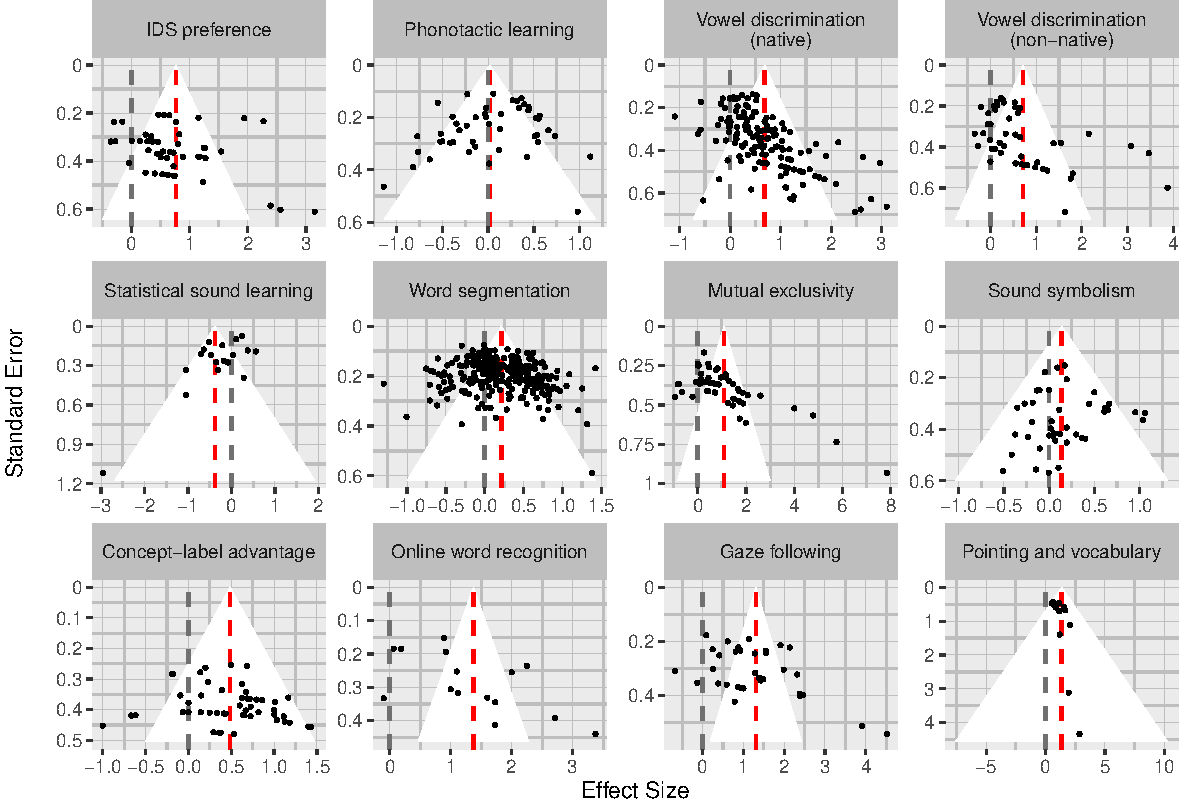
\includegraphics{metalab_synthesis_files/figure-latex/unnamed-chunk-2-1.pdf}
\caption{Funnel plots for each meta-analysis. Each effect size estimate
is represented by a point, and the mean effect size is shown as a red
dashed line. The funnel corresponds to a 95\% (narrow) and 99\% (wide)
CI around this mean. In the absense of true heterogenity in effect sizes
(no moderators) and bias, we should expect all points to fall inside the
funnel.}
\end{figure}

\subsection{P-curves}\label{p-curves}

\begin{figure}[htbp]
\centering
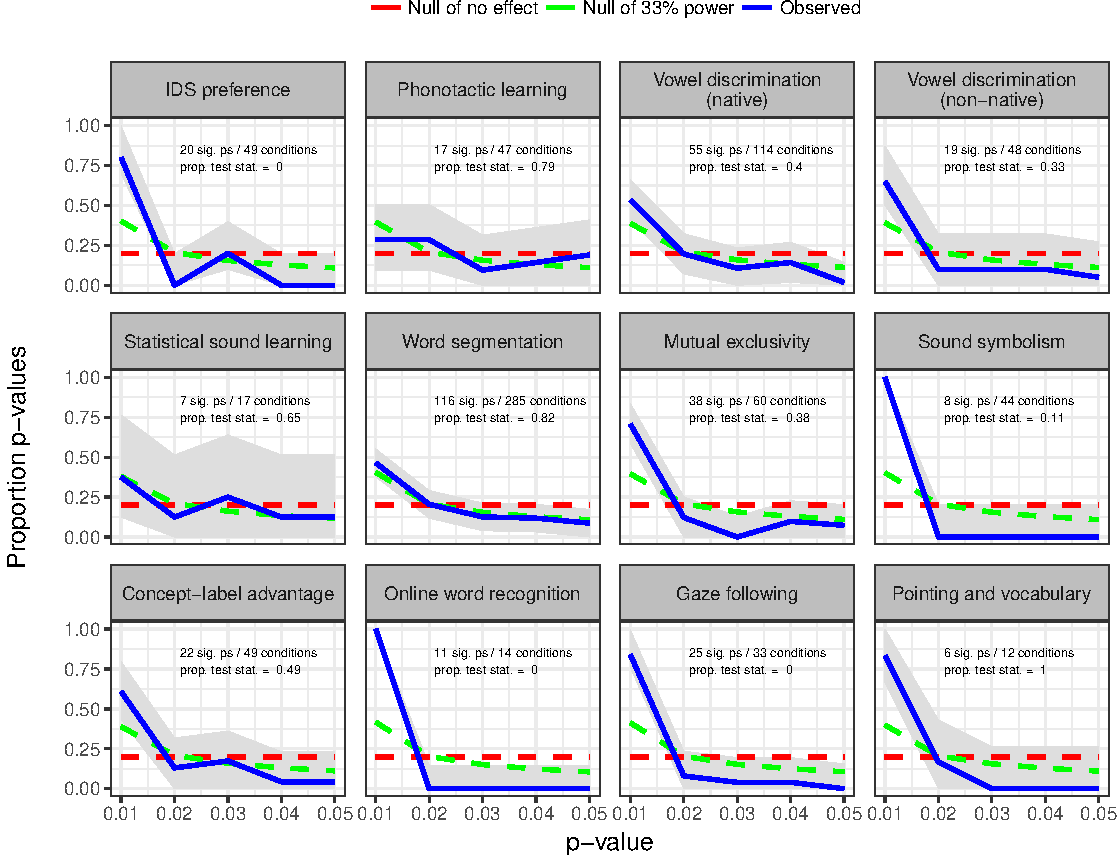
\includegraphics{metalab_synthesis_files/figure-latex/p_curve_plots-1.pdf}
\caption{P-curve for each meta-analysis (Simonsohn, Nelson, \& Simmons,
2014). In the absense of p-hacking, we should expect the observed
p-curve (blue) to be right-skewed (more small values). The red dashed
line shows the expected distribution of p-values when the effect is
non-existent (the null is true). The green dashed line shows the
expected distribution if the effect is real, but studies only have 33\%
power.}
\end{figure}

A p-curve is the distribution of p-values for the statistical test of
the main hypothesis across a literature (Simonsohn et al., 2014b, 2014a,
2015). Critically, if there is a robust effect in the literature, the
shape of the p-curve should reflect this. In particular, we should
expect the p-curve to be right skewed with more small values (e.g., .01)
than large values (e.g., .04). An important property of this analysis is
that we should expect this skew independent of any true heterogeneity in
the data, such as age. Evidence that the curve is in fact right-skewed
would suggest that the literature is not biased, and that it provides
evidential value for theory building.

\begin{table}[t]
\footnotesize
\begin{tabular}{lrrrrr}
\toprule
\textbf{Phenomenon}& \textbf{\textit{d}} & \textbf{fail-safe-N} & \textbf{funnel skew} & \textbf{p-curve skew} & \textbf{power}\\
\midrule
IDS preference & 0.71 [0.53, 0.89] & 3762 & 1.88 (0.06) &  & \\
Phonotactic learning & 0.04 [-0.09, 0.16] & 45 & -1.08 (0.28) & -1.52 (0.06) & 0.14\\
Vowel discrimination (native) & 0.6 [0.5, 0.71] & 9536 & 8.98 (0) & -5.42 (0) & 0.67\\
Vowel discrimination (non-native) & 0.66 [0.42, 0.9] & 3391 & 4.13 (0) & -3.24 (0) & 0.78\\
Statistical sound learning & -0.14 [-0.27, -0.02] & Inf & -1.87 (0.06) &  & \\
Word segmentation & 0.2 [0.15, 0.25] & 5645 & 1.54 (0.12) & -9.67 (0) & 0.56\\
Mutual exclusivity & 1.01 [0.68, 1.33] & 6443 & 6.25 (0) &  & \\
Sound symbolism & 0.15 [0.04, 0.26] & 538 & -1.32 (0.19) & -2.16 (0.02) & 0.96\\
Concept-label advantage & 0.4 [0.29, 0.51] & 3928 & 0.31 (0.76) & -6.15 (0) & 0.69\\
Online word recognition & 1.89 [0.81, 2.96] & 2843 & 2.92 (0) &  & \\
Gaze following & 0.84 [0.26, 1.42] & 2641 & -1.69 (0.09) &  & \\
Pointing and vocabulary & 0.41 [0.32, 0.49] & 1202 & 0.59 (0.55) &  & \\
\bottomrule
\end{tabular}
\caption{Summary of replicability analyses. \textit{d} = Effect size (Cohen's {\it d}) estimated from a random-effect model; fail-safe-N = number of missing studies that would have to exist in order for the overall effect size to be {\it d} = 0; funnel skew = test of asymmetry in funnel plot using the random-effect Egger's test (Stern \& Eggers, 2005); p-curve skew = test of the right skew of the p-curve using the Stouffer method (Simonsohn, Simmons, \& Nelson, 2015); power = power to reject the null hypothesis at the 5\% significance level based on the p-curve (Simonsohn, Nelson, \& Simmons, 2014);  Brackets give 95\% confidence intervals, and parentheses show p-values.}
\end{table}

Figure 2 shows p-curves for 7 of our 12
meta-analyses.\footnote{We did not conduct p-curves on all meta-analyses because previously published meta-analyses did not include test statistics and the key test statistics in some others were inappropriate for p-curve. }
With the exception of phonotactic learning, all p-curves show evidence
of right skew. This is confirmed by formal analyses (Table 2, column 5).

P-curves also provide a method for calculating the overall power of a
literature, based on the shape of the p-curve (Simonsohn et al., 2014a).
Intuitively, when power is high and effect is real, we should be more
likely to observe an effect size \enquote{further} from the null. This
means that we will observe more small effect sizes. Thus, the higher the
power, the more right skewed the p-curve will be. Table 2 (column 6)
presents estimates of power for each meta-analysis based on p-curve.
With the exception of phonotactic learning (\emph{power} = .14),
literatures appear to have acceptable power.

In sum, then, meta-analytic methods, along with our dataset of effect
sizes, provide an opportunity to assess the replicability of the field
of language acquisition. Across a range of analyses, we find that this
literature shows some evidence for bias, but overall, is quite robust.

\section{Theoretical development}\label{theoretical-development}

The replicability analyses suggest that the raw material for theory
building---experimental data---reflect, for the most part, real
psychological phenomena. Given this, we now turn to how these data can
be used to constrain and develop theories of language acquisition.

At the most basic level, meta-analytic methods provide a precise,
quantitative description of the developmental trajectory of individual
phenomena. Figure 3 presents the developmental trajectors of the
phenomena in our dataset at each level in the linguistic
hierarchy.\footnote{The Pointing and Vocabulary dataset is excluded from this analysis because it does not contain effect sizes at multiple ages.}
By describing how effect sizes change as a function of age, we can begin
to understand what factors might moderate that trajectory, such as
aspects of a child's experience or maturation. For example, the mutual
exclusivity meta-analysis suggests a steep developmental trajectory of
this skill. We can use these data to then build quantitative models to
understand how aspects of experience (e.g.~vocabulary development) or
maturational constraints may be related to this trajectory (e.g., M. C.
Frank, Goodman, \& Tenenbaum, 2009; McMurray, Horst, \& Samuelson,
2012).

{[}There are also large differences in the relative magnitude of ES of
different skills. Theoretical point about overt skills have larger ES{]}

But, acquiring a language requires not just learning isolated skills;
acquiring a language is the result of the integration of a range of
skills across the language hierarchy. Consider, for example, a child
understanding the word \enquote{dog:} If the child is unable to segment
\enquote{dog} from natural speech, a child cannot be expected to
understand the meaning of this word. Given these types of
interdependencies, we can therefore usefully think of language
acquisition as a \emph{system} where different skills interact and
depend on each other. In building a theory of this system, a pragmatic
and necessary research strategy has been to study these skills primarily
in isolation, describing the developmental trajectory of individual
phenomena in separate research programs. However, if it is indeed the
case that there are dependencies between these skills, then we may not
be able to ultimately understand one skill without having a more
complete picture of other skills, as well as a common language for
talking about their relationship.

\begin{figure}[htbp]
\centering
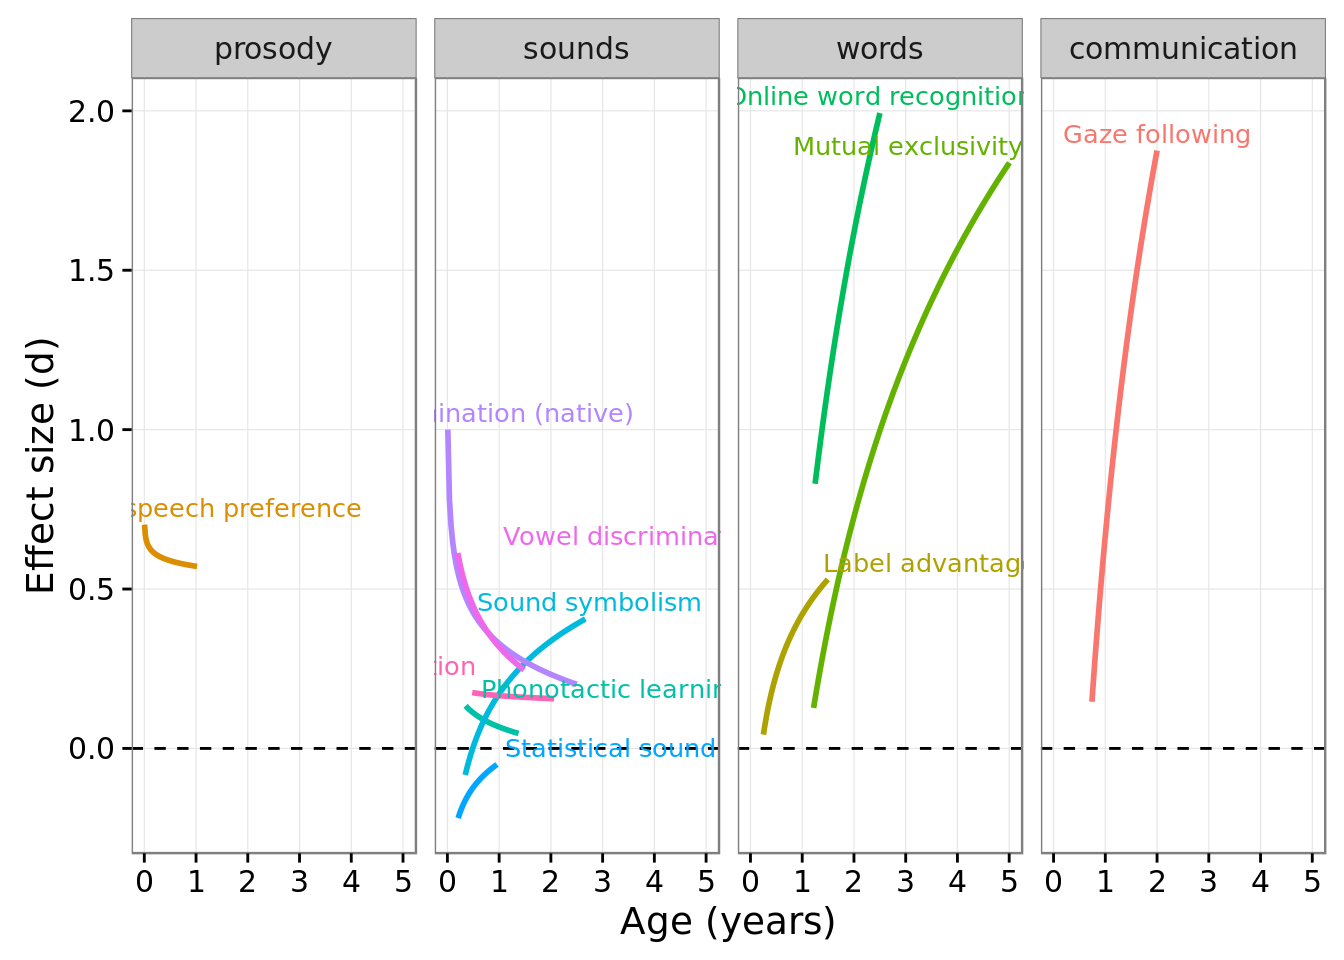
\includegraphics{metalab_synthesis_files/figure-latex/unnamed-chunk-4-1.pdf}
\caption{Effect size plotted as a function of age across all
developmental meta-analyses in our dataset. Lines show logarithmic model
fits.}
\end{figure}

A useful analogy is thermodynamic processes in weather. A meteorologist
can carefully describe changes in temperature over the course of a day
in a particular location. But, to explain and predict those changes, the
meteorologist needs to know about other variables in the system, like
atmospheric pressure. Quantitative models can then be applied to
understand the relationship between the two. Similarly, to predict and
explain a child's understanding of the word \enquote{dog,} we need not
only to describe the child's competency in understanding this word, but
also the child's competency in other skills like phonemic knowledge,
word segmentation, and pragmatic reasoning. Like in the case of
thermodynamics, quantitative methods provide a rich toolkit for relating
these phenomena

\begin{figure}[htbp]
\centering
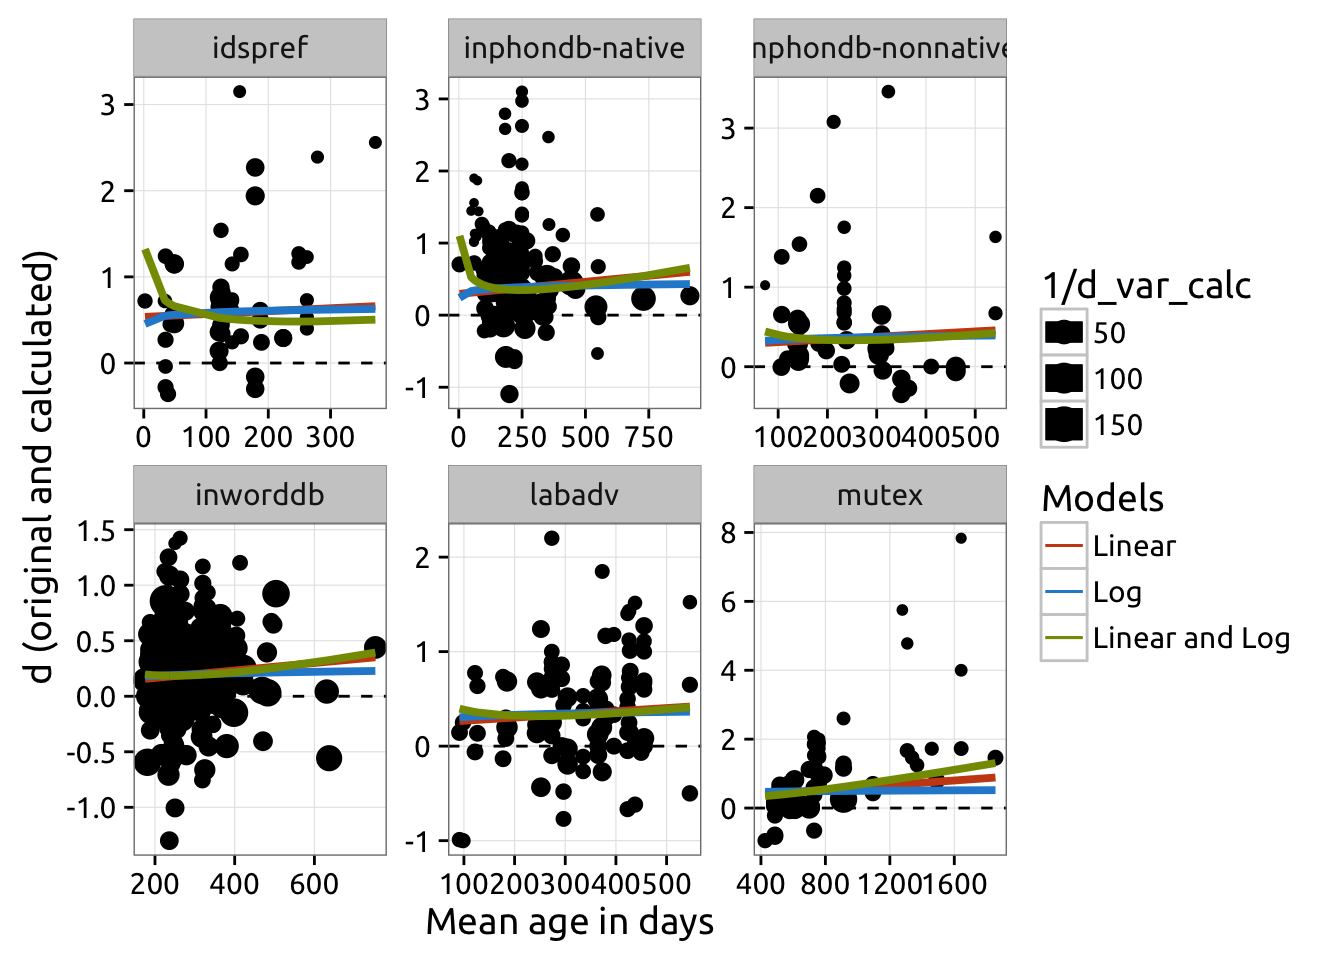
\includegraphics{metalab_synthesis_files/figure-latex/unnamed-chunk-5-1.pdf}
\caption{Effect size as a function of age from 0-3 years, across 11
different phenomena. Each point corresponds to a condition, with the
size of the point indicating the number of participants. Models show
logarithmic fits. These developmental curves suggest there is
interactivity across language skills, rather than sequential learning of
the linguistic hierarchy}
\end{figure}

We suggest that meta-analytic methods provide an approach for
synthesizing across different linguistic skills via the language of
effect sizes. The ultimate goal is to use meta-analytic data to build a
single, quantitative model of the language acquisition system, much like
those developed for individual language acquisition phenomena, like word
learning. Developing a single quantitative model is a lofty goal,
however, and will likely require much more precise description of the
phenomena than is available in our dataset. Nevertheless, we can use our
data to distinguish between broad meta-theories about the relationship
between different skills.

There are two existing meta-theories in the literature about the
dependencies between different skills in language acquisition. The
first---the ``bottom-up" theory---proposes that linguistic skills are
acquired sequentially beginning with skills at the lowest level of the
linguistic hierarchy. Under this theory, once a skill is mastered, it
can be used to support the acquisition of skills higher in the
linguistic hierarchy. In this way, a child sequentially acquires the
skills of language, \enquote{bootstrapping} from existing knowledge at
lower levels to new knowledge at higher levels. There is a wide range of
evidence consistent with this view. For example, there is evidence that
prosody supports the acquisition of sound categories {[}CITE{]}, word
boundaries {[}CITE{]}, and even word learning (e.g., Shukla, White, \&
Aslin, 2011).

A second possibility is that there is interactivity in the language
system such that multiple skills are learned simultaneously across the
system. Under this proposal, a child does not wait to begin learning the
meanings of words until the sounds of a language are mastered, for
example; rather, the child is jointly solving the problem of word
learning in concert other language skills. This possibility is
consistent with predictions of a class of hierarchical Bayesian models
that suggest that more abstract knowledge may be acquired quickly,
before lower level information, and may in turn support the acquisition
of lower information (``Blessing of abstraction,'' Goodman, Ullman, \&
Tenenbaum, 2011). There is evidence for this proposal from work that
that suggests word learning is supported the acquisition of lower-level
information like phonemes (Feldman, Myers, White, Griffiths, \& Morgan,
2013). More broadly, there is evidence that higher level skills like
word learning may be acquired relatively early in development, likely
before lower level skills have been mastered (e.g., Bergelson \&
Swingley, 2012)

Within the meta-analytic framework of effect-sizes, we can represent
these two theories schematically in figure 4a (bottom-up) and 4b
(interactive) {[}A figure here?{]}. This framework also allows us to
specify a much larger space of possible theories, however. By specifying
several parameters of the framework, such as the shape of the
developmental trajectory (e.g., linear or logarithmic), direction of the
trajectory (upward or downward) and the age at which acquisition begins,
we can consider many possible meta-theories of development.

Our data allow us to begin to differentiate between this space of
theories. Figure 5 presents a holistic representation of the
developmental trajectories of all the skills in our dataset. We find
strong evidence for interactivity---children begin learning even
high-level skills like the meanings of words early on in development,
and even low-level skills like sound categories show a protracted period
of development. Moving forward, we can use this approach to distinguish
between a larger space of meta-theories and, ultimately, build a single
quantitative theory of language acquisition.

\section{Discussion}\label{discussion}

Building a theory of a complex psychological phenomenon requires making
good inductive inferences from the available data. We suggest that
meta-analysis can support this process by allowing the researcher to
verdically describe the to-be-explained behavior, and to do so with
high-fidelity. Here, we apply the meta-analytic toolkit to the domain of
language acquisition---a domain where there are concerns of
replicability, and where high-fidelity data is needed to explain its
complexity. We find that the existing literature in this domain describe
robust phenomena and thus should form the basis of theory development.
We then offer a preliminary synthesis of the field by aggregating across
language acquisition phenomena. We find evidence that linguistic skills
are acquired interactively rather than in a strictly bottom-up fashion.

There are a number of important limitations to the meta-analytic
approach as a theoretical tool. First, this method relies on researchers
conducting replications of the same study across a range of ages and,
critically, reporting these data so that they can be used in
meta-analyses. To the extent that researchers do not conduct these
studies, or report the necessary statistics in their write-ups (e.g.,
means and standard deviations), the meta-analytic method cannot be
applied. Second, the meta-analytic method, as for qualitiative forms of
synthesis (e.g.~literature review), is limited by the potential presence
of bias, which can come from a ranges of sources including
non-representative participant populations, failure to publish null
findings, and analytical degrees-of-freedom. To the extent these biases
are present in the literature, methods of synthesizing these findings
will also be biased.

In addition, there are a number of more substantive concerns with this
method. One possibility is that the magnitude of effect may be more
related to the method than the psychological phenomenon. While this may
be true to some extent, we find that method does not have a large impact
on effect size for a phenomena, relative to other moderators like age
(see SI). Another issue is that meta-analysis usually measures signal to
noise, not units of interest (e.g.~ability in an absolute sense), so
there could be important confounds with respect to this.

Future directions:

\begin{itemize}
\item
  Educational tool - presage/link to other paper
\item
  Contributions, CAMAS
\item
  Other domains -- language acquistion as a case study
\end{itemize}

\paragraph{Author Contributions}\label{author-contributions}

\paragraph{Acknowledgments}\label{acknowledgments}

\newpage

\subsubsection{References}\label{references}

\setlength{\parindent}{-0.5in} \setlength{\leftskip}{0.5in}
\setlength{\parskip}{8pt}

\hypertarget{refs}{}
\hypertarget{ref-anderson2016response}{}
Anderson, C. J., Bahník, Š., Barnett-Cowan, M., Bosco, F. A., Chandler,
J., Chartier, C. R., \ldots{} others. (2016). Response to comment on
``estimating the reproducibility of psychological science''.
\emph{Science}, \emph{351}(6277), 1037--1037.

\hypertarget{ref-bergelson2016}{}
Bergelson, E., \& Swingley, D. (2012). At 6--9 months, human infants
know the meanings of many common nouns. \emph{Proceedings of the
National Academy of Sciences}, \emph{109}(9), 3253--3258.

\hypertarget{ref-bergmann2015development}{}
Bergmann, C., \& Cristia, A. (2015). Development of infants'
segmentation of words from native speech: A meta-analytic approach.
\emph{Developmental Science}.

\hypertarget{ref-dunst2012preference}{}
Dunst, C., Gorman, E., \& Hamby, D. (2012). Preference for
infant-directed speech in preverbal young children. \emph{Center for
Early Literacy Learning}, \emph{5}(1).

\hypertarget{ref-feldman2013word}{}
Feldman, N. H., Myers, E. B., White, K. S., Griffiths, T. L., \& Morgan,
J. L. (2013). Word-level information influences phonetic learning in
adults and infants. \emph{Cognition}, \emph{127}(3), 427--438.

\hypertarget{ref-frank2009using}{}
Frank, M. C., Goodman, N. D., \& Tenenbaum, J. B. (2009). Using
speakers' referential intentions to model early cross-situational word
learning. \emph{Psychological Science}, \emph{20}(5), 578--585.

\hypertarget{ref-frank2016performance}{}
Frank, M. C., Lewis, M. L., \& MacDonald, K. (in press). A performance
model for early word learning. In \emph{Proceedings of the 38th Annual
Conference of the Cognitive Science Society}. Retrieved from
\url{http://langcog.stanford.edu/papers_new/frank-2016-underrev.pdf}

\hypertarget{ref-Gilbert1037}{}
Gilbert, D. T., King, G., Pettigrew, S., \& Wilson, T. D. (2016).
Comment on Estimating the reproducibility of psychological science.
\emph{Science}, \emph{351}(6277), 1037--1037.
doi:\href{https://doi.org/10.1126/science.aad7243}{10.1126/science.aad7243}

\hypertarget{ref-goodman2011learning}{}
Goodman, N. D., Ullman, T. D., \& Tenenbaum, J. B. (2011). Learning a
theory of causality. \emph{Psychological Review}, \emph{118}(1), 110.

\hypertarget{ref-ioannidis2005most}{}
Ioannidis, J. P. (2005). Why most published research findings are false.
\emph{PLoS Med}, \emph{2}(8), e124.

\hypertarget{ref-lfprep}{}
Lewis, M., \& Frank, M. C. (in prep). Multiple routes to disambiguation.

\hypertarget{ref-mcmurray2012word}{}
McMurray, B., Horst, J. S., \& Samuelson, L. K. (2012). Word learning
emerges from the interaction of online referent selection and slow
associative learning. \emph{Psychological Review}, \emph{119}(4), 831.

\hypertarget{ref-open2012open}{}
Open Science Collaboration. (2012). An open, large-scale, collaborative
effort to estimate the reproducibility of psychological science.
\emph{Perspectives on Psychological Science}, \emph{7}(6), 657--660.

\hypertarget{ref-open2015estimating}{}
Open Science Collaboration. (2015). Estimating the reproducibility of
psychological science. \emph{Science}, \emph{349}(6251), aac4716.

\hypertarget{ref-orwin1983fail}{}
Orwin, R. G. (1983). A fail-safe n for effect size in meta-analysis.
\emph{Journal of Educational Statistics}, 157--159.

\hypertarget{ref-Peterson:2016}{}
Peterson, D. (2016). The Baby Factory: Difficult Research Objects,
Disciplinary Standards, and the Production of Statistical Significance.
\emph{Socius: Sociological Research for a Dynamic World}, \emph{2}(0),
1--10.

\hypertarget{ref-shukla2011prosody}{}
Shukla, M., White, K. S., \& Aslin, R. N. (2011). Prosody guides the
rapid mapping of auditory word forms onto visual objects in 6-mo-old
infants. \emph{Proceedings of the National Academy of Sciences},
\emph{108}(15), 6038--6043.

\hypertarget{ref-simonsohn2014power}{}
Simonsohn, Nelson, L. D., \& Simmons, J. P. (2014a). P-curve and effect
size correcting for publication bias using only significant results.
\emph{Perspectives on Psychological Science}, \emph{9}(6), 666--681.

\hypertarget{ref-simonsohn2014p}{}
Simonsohn, Nelson, L. D., \& Simmons, J. P. (2014b). P-curve: A key to
the file-drawer. \emph{Journal of Experimental Psychology: General},
\emph{143}(2), 534.

\hypertarget{ref-simonsohn2015better}{}
Simonsohn, Simmons, J. P., \& Nelson, L. D. (2015). Better p-curves.
\emph{Simonsohn, Uri, Joseph P. Simmons, and Leif D. Nelson
(Forthcoming),``Better P-Curves,'' Journal of Experimental Psychology:
General}.

\hypertarget{ref-sterne2005regression}{}
Sterne, J. A., \& Egger, M. (2005). Regression methods to detect
publication and other bias in meta-analysis. \emph{Publication Bias in
Meta-Analysis: Prevention, Assessment, and Adjustments}, 99--110.

\hypertarget{ref-tsuji2014perceptual}{}
Tsuji, S., \& Cristia, A. (2014). Perceptual attunement in vowels: A
meta-analysis. \emph{Developmental Psychobiology}, \emph{56}(2),
179--191.



\end{document}
